% !TEX root = main.tex
%%%%%%%%%%%%%%%%%%%%%%%%%%%%%%%%%%%%%%%%
%%%%%%%%%%%%%%%%%%%%%%%%%%%%%%%%%%%%%%%%
\section{Results Discussion} \label{sec:results}
%%%%%%%%%%%%%%%%%%%%%%%%%%%%%%%%%%%%%%%%
%%%%%%%%%%%%%%%%%%%%%%%%%%%%%%%%%%%%%%%%

We start by contrasting the performances of LEONID and LANCE (\secref{sec:rq1}). We follow the quantitative analysis by presenting qualitative examples of partially correct predictions in which only the log message synthesized by LEONID is wrong, while the other information (\ie variable, log level, position) are correctly predicted, but still meaningful as suggestion for developers. Then, we outline the results achieved by LEONID when injecting multiple log statements (\secref{sec:rq2}). Finally, \secref{sec:rq3} presents the results achieved by LEONID when deciding whether or not log statements are needed in a given \java method.


\subsubsection{Performance of LEONID in injection single complete log statements in \java methods (RQ$_{1}$)}
\label{sec:rq1}

\tabref{tab:single-train-results} reports the results achieved by the LEONID and LANCE, in terms of correct and partially correct predictions. We report the correct predictions for all combinations of the four ``components'' to predict (\ie log variable, log level, position where to inject it, and log message). To this extent, we analyze cases in which both LEONID and LANCE managed to correctly inject a log statement in a \java method and cases in which  at least one of the four components to predict was correct (\ie partially correct prediction).
To facilitate the reading of \tabref{tab:single-train-results}, we briefly explain how to symbols featuring it.
Each row can includes only two out of three symbols: (i) the check mark (\cmark) indicates that the results reported in that row refer to log statements in which the component ($c$) was correctly predicted. The dash mark ($-$), instead, indicates that $c$ can be either correct or wrong for the predictions in that row. Finally, the cross mark (\xmark) indicates that the component was wrongly predicted for the corresponding log statements.
For instance, the last row of \tabref{tab:single-train-results} reports the results achieved by LEONID and LANCE, when the two models correctly synthesized the log variable name, the log level and the entire the log statement has been injected in the correct position. In such a case however, the log message has been wrongly predicted, as it can be seen thanks the cross mark (\xmark) in the log message column.

The last two columns of \tabref{tab:single-train-results} report the $p$-value and the Odds Ratio (OR) effect size we compute using the Mc-Nemar's test \cite{mcnemar}.

By Comparing the correct predictions (\ie first row of \tabref{tab:single-train-results}) achieved by LEONID and LANCE, it emerges that LEONID performs slightly better than LANCE, achieving 27.26\% of correct predictions against 26.79\% achieved by LANCE. As it can be seen, the (adjusted) $p$-value indicates a statistically significant difference, with LEONID having 1.12 higher odds of providing a correct prediction compared to LANCE. 
As for the other ``components'', what emerges is that LEONID performs slightly worse compared to LANCE.
This is true, especially for the log variable name, the log level, and, when considering, both components along with the log position (\ie last raw of \tabref{tab:single-train-results}). 
In these cases, the (adjusted) $p$-values indicate a statistically significant difference with ORs ranging between 0.80 to 0.91 in favor of LANCE. Concerning the log messages and the position where the log statements have been injected, LEONID performs better than LANCE.
In detail, we found out that LEONID can generate 31.55\% of correct log messages while LANCE achieves 30.16\% of correct generated log messages. The Mc-Nemar's test computed for such component indicates a statistically significant difference ($p$-value $<$ 0.01), with LEONID being 1.36 more likely than LANCE when generating a log message as a real developer would do.

For the position of log statements, the difference between the two models are almost negligible. To this extent, LEONID can correctly injects log statements in \java method in 82.35\% of cases as compared to LANCE, which achieves 82.28\%. Such small differences are also captured by the statistical test we performed, for which the high $p$-value of 0.71 fails in pointing out any statistically significant difference between the two distributions.

As for the quality of the log messages, \tabref{tab:log-messages-stats} reports the results computed using the four NLP metrics presented in (\secref{sec:design}) for both models: LANCE and LEONID. For the latter, we report the results when different coding contexts (\ie $k=1$, $k=3$ and $k=5$) are used. 

In detail, we first report the BLEU score computed at corpus level, then we also report the METEOR metric and to conclude the ROUGE-LCS metric and the LEVENSHTEIN distance complement the set of NLP-related metrics we decide to use for evaluating the quality of the log messages.

By analyzing \tabref{tab:log-messages-stats}, the first thing that leap to eyes is the difference in terms of BLEU-A when comparing the performances achieved by LANCE against LEONID. In particular, as the coding context increases, such a difference tends to become more pronounced, with gains ranging between 2.8 to 3.6 percentage points in favor of LEONID. A similar trend is found when looking at different overlapping $n$-grams (\ie BLEU-1, BLEU-2, BLUE-3 and BLEU-4). 

Focusing on the METEOR score, we found LEONID to generate log messages that are more likely to be perceived of higher quality by humans \cite{meteor}, as compared to LANCE, with scores that, on average, are 1.5\% higher. We speculate that such a result is the consequence of force-feeding the model with log messages from which it can learn and thus recommend more meaningful log messages.

As for the ROUGE-LCS, it emerges that when augmenting the input instances with log messages coming from the training set, the performances achieved by LEONID with different coding context, are always higher than LANCE, with the highest value of 44.33 points achieved with a coding context of $k=5$ as compared to 42.19 points obtained by LANCE.

Finally, the Normalized LEVENSHTEIN distance indicates how log messages produced by LEONID ($k=5$) would require up to 41.85\% of changes to match the ones written by developers. If contrasting such a result with the LEVENSHTEIN distance computed for LANCE, we realize that (on average) the number of words that a developer is asked to change is 44.02\% higher when using LANCE as compared to LEONID.

We complement the discussion of the NLP-related metrics by performing the Wilcoxon signed-rank test \cite{wilcoxon}, adjusting $p$-values to account for multiple comparisons using the Holm's correction procedure \cite{Holm1979a}. 
From the results we report in \tabref{tab:test-wilcoxon}, it comes to light how, for each metric, we always have a difference statistically significant, with a negligible effect size for all the metrics, in favor of LEONID (for the Levenshtein distance a positive d is in favor of LEONID, as it is a distance). 

Concerning the qualitative analysis, among the 300 partially correct predictions analyzed for LEONID, we found 198 of them (66\%) to report the same information of the target. In other words, the recommended log message was different but semantically equivalent to the target (\ie oracle). The remaining 102 (34\%) predictions, reported a log message different or not meaningful as compared to the target. 
For LANCE, we found 192 (64\%)  partially correct predictions to report a meaningful log message, with 108 (36\%) of them being considered as not meaningful.
Such result confirms the finding of Mastropaolo \etal \cite{mastropaolo2022using}, meaning that a strict quantitative evaluation would produce misleading results, especially when narrowing down the focus only on the correct predictions. 
Furthermore, the bigger code base (almost twice as bigger) that we leveraged to train LANCE and LEONID produced a substantial effect in boosting the performances of both models on each experimented metric, with a qualitative evaluation that allowed us to estimate a 66\% and 64\% of predictions still valuable when using LEONID and LANCE respectively.

To give a better understanding to the reader of such cases, \figref{} reports .... \TODO{LUCA please continue here}



%if we have space put this back
%\begin{figure*}[h]
%	\centering
%	\label{fig:rq1-message-stats}
%	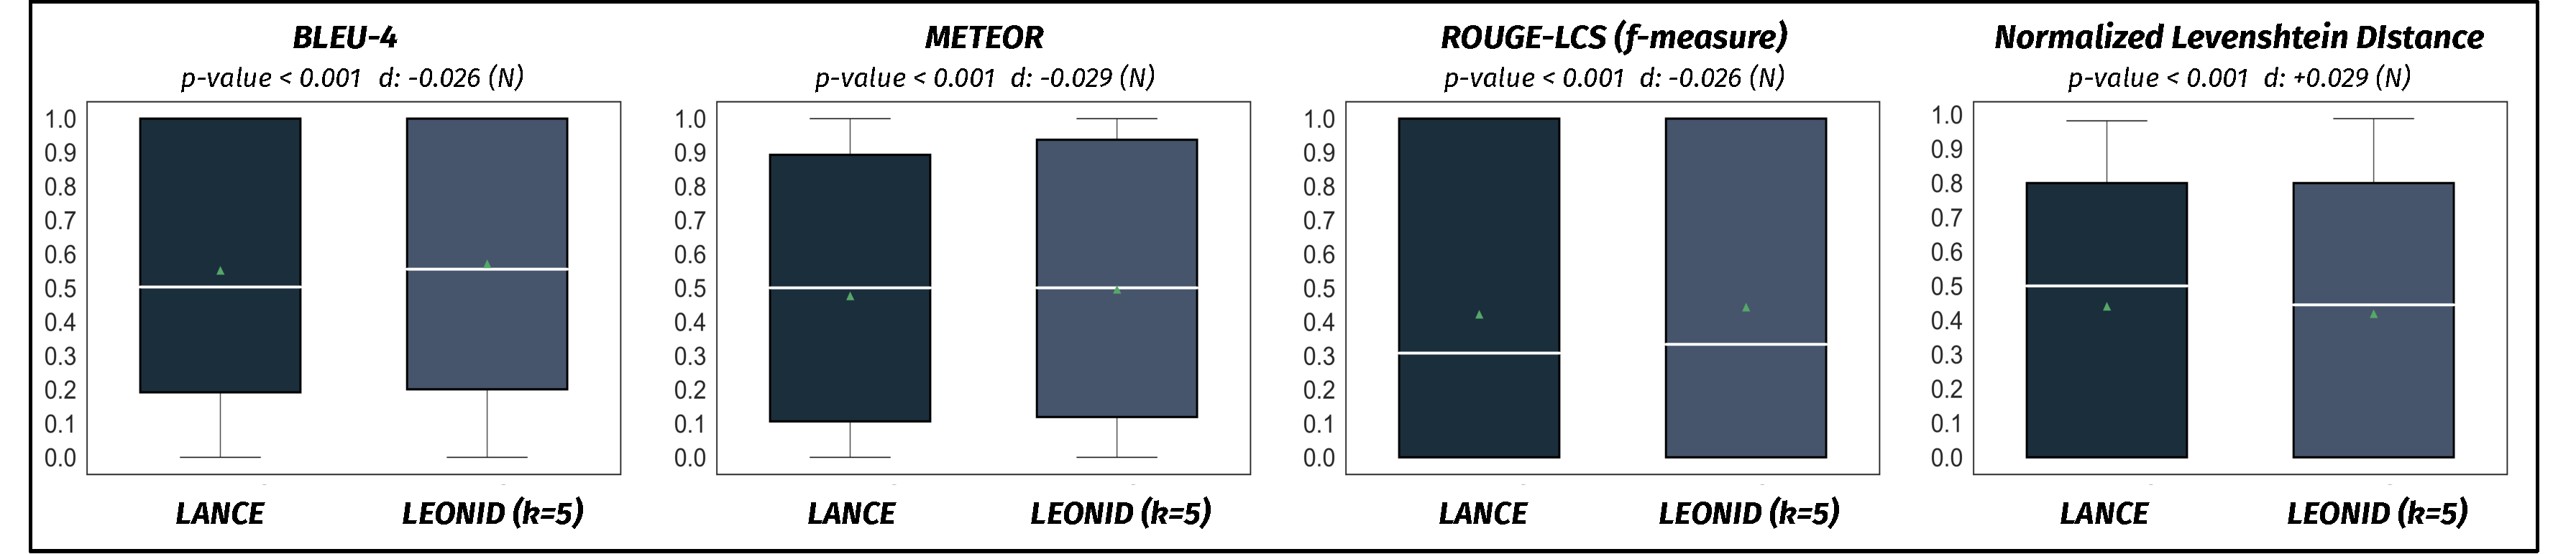
\includegraphics[width=\textwidth]{img/RQ1-log-message-boxplot.pdf}
%	\caption{Characteristics of log messages synthesized by LANCE and LEONID (K=5)}
%\end{figure*}



\begin{table}[h!]
  \centering
  \caption{Correct predictions considering the four-dimensional challenges of injecting log statements.}
  \resizebox{.5\textwidth}{!}{
	  \begin{tabular}{cccccrrrr}
	  \hline
	  Variable   & Level     & Message   & Position  &  & \multicolumn{1}{c}{LEONID} & \multicolumn{1}{c}{LANCE} & \multicolumn{1}{c}{$p$-value} & \multicolumn{1}{c}{OR}     \\ \hline
	  \ding{51}  & \ding{51} & \ding{51} & \ding{51} &  & 27.26\%                    & 26.78\%                   &                           &                            \\
	  \ding{51}  & -         & -         & -         &  & 76.45\%                    & 77.15\%                   &                           &                            \\ 
	  -          & \ding{51} & -         & -         &  & 73.53\%                    & 74.18\%                   &                           &                            \\
	  -          & -         & \ding{51} & -         &  & 31.55\%                    & 30.16\%                   &                           &                            \\ 
	  -          & -         & -         & \ding{51} &  & 82.35\%                    & 82.28\%                   &                           &                            \\ \hline
	  \ding{51}  & \ding{51} & \ding{55} & \ding{51} &  & 28.14\%                    & 29.86\%                    &                           &                            \\ \hline 
	  
	  \end{tabular}
  }
  \label{tab:single-train-results}
\end{table}





\begin{table}[h]
	\centering
	\caption{Evaluation Metrics on Log Messages: LEONID \emph{vs} LANCE\vspace{-0.2cm}}
	\scriptsize
	\label{tab:log-messages-stats}
	 \resizebox{.5\textwidth}{!}{
	\begin{tabular}{lrrrrrr}
		\toprule
		& {\bf LANCE} & {\bf LEONID ($k=1$)} &  {\bf LEONID ($k=3$)} &  {\bf LEONID ($k=5$)} \\\midrule
		BLEU-A \cite{papineni2002bleu}& 31.98 & 34.86  & 35.07 & \bf 35.36\\
			\hspace{0.2cm} BLEU-1 & 47.30 &  49.10 & 49.70  & \bf 50.00\\
			\hspace{0.2cm} BLEU-2 & 36.30 & 38.70 & 39.20 & \bf 39.60\\
			\hspace{0.2cm} BLEU-3 & 33.90 &  33.53 & 34.50 & \bf 35.00\\
			\hspace{0.2cm} BLEU-4 & 31.40 & 33.53 & 31.80 & \bf 32.40\\
		METEOR \cite{meteor} & 58.60 & 60.03  & \bf 60.43 & 60.35 \\
		ROUGE-LCS \cite{lin2004rouge} &  &  & & \\
		\hspace{0.2cm} $precision$ & 42.57 & 44.67 & 44.51  & \bf 44.68\\
		\hspace{0.2cm} $recall$ & 44.04 &  45.94 & 45.80 & \bf 46.01\\
		\hspace{0.2cm} $fmeasure$ & 42.19 & 44.26 & 44.14 & \bf 44.33\\
		LEVENSHTEIN \cite{levenshtein1966} & 44.02 & 42.27  & 41.91 & \bf 41.85 \\\bottomrule
	\end{tabular} 
	\vspace{-0.2cm}
}
\end{table}

\begin{table}[ht]
	\centering
	\caption{Statistical Tests: LEONID \emph{vs} LANCE\vspace{-0.2cm}}
	\scriptsize
	\label{tab:test-wilcoxon}
	 \resizebox{.5\textwidth}{!}{
	\begin{tabular}{llrc}
		\toprule
		\textbf{Comparison} & \textbf{Metric} & \textbf{\emph{p}-value} & \textbf{d} \\ 
		\midrule
		\multirow{3}{*}{LANCE  \emph{vs} LEONID ($k=1$)} & BLEU-4 & $<$0.001 & -0.022 (N) \\ 
			& METEOR & $<$0.001 & -0.025 (N) \\
		& ROUGE-LCS (f-measure) & $<$0.001 & -0.025 (N) \\ 
		& LEVENSHTEIN & $<$0.001 & +0.023 (N) \\\midrule
		\multirow{3}{*}{LANCE  \emph{vs} LEONID ($k=3$)} & BLEU-4 & $<$0.001 & -0.026 (N) \\ 
		& METEOR & $<$0.001 & -0.029 (N) \\
		& ROUGE-LCS (f-measure) & $<$0.001 & -0.023 (N) \\ 
		& LEVENSHTEIN & $<$0.001 & +0.027 (N) \\\midrule
			\multirow{3}{*}{LANCE  \emph{vs} LEONID ($k=5$)} & BLEU-4 & $<$0.001 & -0.026 (N) \\ 
		& METEOR & $<$0.001 & -0.029 (N) \\
		& ROUGE-LCS (f-measure) & $<$0.001 & -0.026 (N) \\ 
		& LEVENSHTEIN & $<$0.001 & +0.029 (N) \\\midrule
	\end{tabular}
}
	\vspace{-0.2cm}
\end{table}


\subsubsection{Performance of LEONID in injection multiple complete log statements in \java methods (RQ$_{2}$)}
\label{sec:rq2}
As explained in \secref{sec:design}, for RQ$_{2}$ we would not be able to compute the partially correct predictions as we performed for RQ$_{1}$. For such a reason, we limit our discussion presenting the results achieved by LEONID when injecting multiple log statements in \java Methods, while reporting qualitative examples in our online appendix \cite{}. To this extent, we found out LEONID to correctly inject multiple log statements in \java methods in 23.38\% (5,634 out of 24,088) when using a ``shallow'' coding context $k=1$. Similarly, even when increasing the window of the coding context (\ie $k=3$ and $k=5$), the achieved results do not undergo major changes, with 23.35\% for $k=3$ and 23.51\% for $k=5$.


\subsubsection{Performance of LEONID in properly deciding whether or not a \java method needs log statements  (RQ$_{3}$)}
\label{sec:rq3}

\figref{fig:rq3-cm} reports the confusion matrices with their respective values of accuracy, precision and recall (on the bottom of the figure) for each test-set in \tabref{tab:ds-summary-2}.

When half of the methods need at least one log statement, and the other half do not need any (50-50 split), LEONID reports an accuracy of 0.96 while achieving a precision of 0.98 and a recall of 0.94. In contrast the \textit{optimistic} and \textit{pessimistic} classifier would achieve 0.50 of accuracy and precision, while reporting a recall of 1.0. 
The \textit{random} classifier on the same test-set (50-50), achieves 0.50 of accuracy, precision, and recall (as expected). 

When testing LEONID on the 75-25 split, there is a slightly increase in terms of precision as compared to the 50-50 split, 0.98 \emph{vs} 0.99. Consequently, the accuracy loose 0.01 points (0.95) as compared to the previous 50-50 split. Instead, the recall keeps its value fixed at 0.94.
The \textit{optimistic} classifier reports a value of 0.75 for both accuracy and precision, while achieving a recall of 1.0. As expected, the \textit{pessimistic} classifier achieves 0.25 points for both accuracy and precision and, 1.0 of recall. As for the \textit{random} classifier, we found out an accuracy and a recall of 0.5, with a precision of 0.75.

When LEONID is tested in a scenario where the number of methods requiring log statements is outweighed by the number of methods that do not need log statements (25-75 split), precision and recall achieve both 0.94. The accuracy for such a scenario is 0.97. 
On the other hand, the \textit{optimistic} classifier would achieve a recall of 1.0, with accuracy and precision both of 0.25, which contrasts the results achieved with the \textit{pessimistic} classifier, which would report a recall of 1.0,  with accuracy and precision of 0.75. On such dataset, the \textit{random} classifier would ensure a precision of 0.25, with accuracy and recall of 0.50.

Finally, as for the test-set resembling the original distribution of \java methods we mined (2-98 split), LEONID achieves an accuracy of 0.98 and a recall of 0.96. Instead, the precision goes down to 0.51.
As for the naive classifiers, we found out that when using the \textit{optimistic}, the achieved accuracy and precision would be both 0.02 points, with a recall of 1.0.
In contrast, the \textit{pessimistic} performs better than LEONID (as expected), achieving 0.97 for both accuracy and precision, and 1.0 for recall.
The \textit{random} classifier, on the other hand, would ensure accuracy of 0.50, and a recall of 0.53, while achieving only 0.02 of precision.


\begin{table}[ht]
	\centering
	\caption{Statistical Tests: LEONID \emph{vs} NAIVE Classifiers\vspace{-0.2cm}}
	\scriptsize
	\label{tab:statistical-classifier}
	\resizebox{.5\textwidth}{!}{
		\begin{tabular}{llrc}
			\toprule
			\textbf{Test Set} & \textbf{Metric} & \textbf{\emph{p}-value} & \textbf{OR} \\ 
			\midrule
			\multirow{3}{*}{Need4Log: (50-50)} 
			& Optimistic \emph{vs} LEONID & $<$0.001 &18.57 \\ 
			& Pessimistic \emph{vs} LEONID & $<$0.001 & 50.28 \\ 
			& Random \emph{vs} LEONID & $<$0.001 & 27.12 \\\midrule
			\multirow{3}{*}{Need4Log: (75-25)} 
			& Optimistic \emph{vs} LEONID & $<$0.001 & 6.17 \\ 
			& Pessimistic \emph{vs} LEONID & $<$0.001 & 140.43 \\ 
			& Random \emph{vs} LEONID & $<$0.001 & 21.41 \\\midrule
			\multirow{3}{*}{Need4Log: (25-75)} 
			& Optimistic \emph{vs} LEONID & $<$0.001 & 54.58 \\ 
			& Pessimistic \emph{vs} LEONID & $<$0.001 & 16.73 \\ 
			& Random \emph{vs} LEONID & $<$0.001 & 33.77 \\\midrule
			\multirow{3}{*}{Need4Log: (2-98)} 
			& Optimistic \emph{vs} LEONID & $<$0.001 & 1,426 \\ 
			& Pessimistic \emph{vs} LEONID & 0.63 & 1.05 \\ 
			& Random \emph{vs} LEONID & $<$0.001 & 56.53 \\\midrule
		\end{tabular}
	}
	\vspace{-0.2cm}
\end{table}


The results of the statistical comparison made using McNemar’s test are reported in \tabref{tab:statistical-classifier}.
As it is shown, LEONID has a positive (OR$>$1) and statistically significant effect in all cases but one. When testing LEONID against the Need4Log (2-98) dataset, we found that for the comparison \textit{Pessimistic} \emph{vs} LEONID, although the OR$>$1, the $p$-value of 0.63 points out to a non statistically significant effect. Such a results is indeed expected, seen the distribution of the labels (\ie \textit{Need}, \textit{No need}) featuring the Need4Log (2-98) dataset. 


\begin{figure*}[h!]
	\centering
	\label{fig:rq3-cm}
	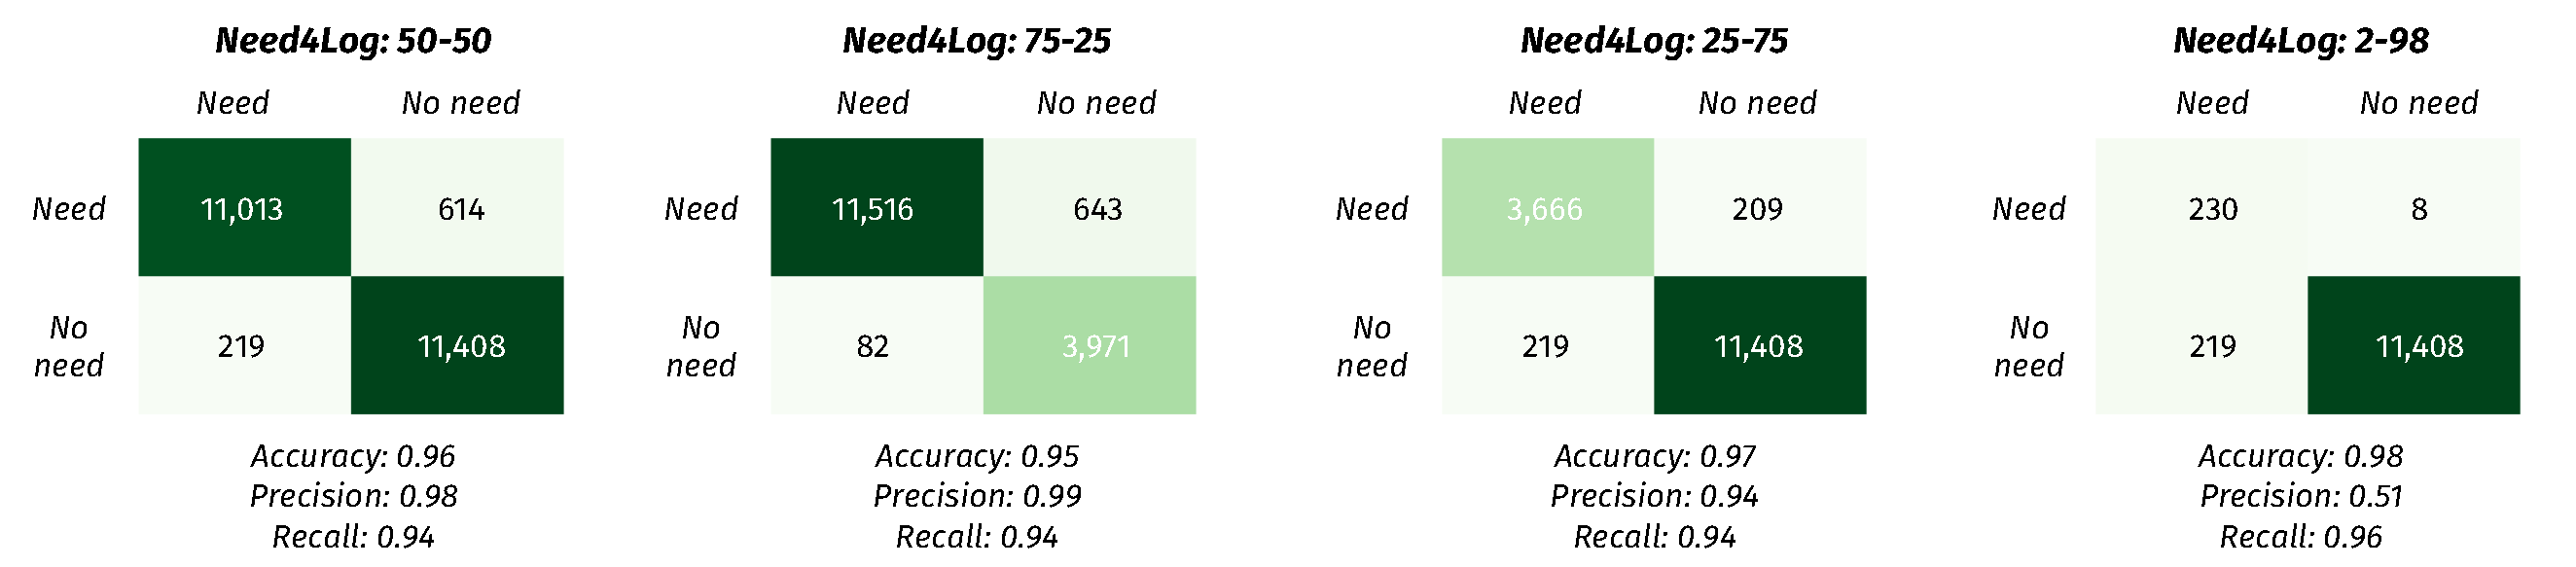
\includegraphics[width=\textwidth]{img/RQ3-CM.pdf}
	\caption{Results achieved by LEONID when deciding whether log statements are needed or not in \java methods. For each test-set (\tabref{tab:ds-summary-2}), accuracy, precision and recall are reported.}
\end{figure*}



%complementarity
%Shared:  72.05602393255371
%Only LEONID:  14.781071525700298
%Only LANCE:  13.162904541745988

